\documentclass[11pt,a4paper]{article}
\usepackage[T1]{fontenc}
\usepackage{lmodern}
\usepackage[margin=1in]{geometry}
\usepackage{amsmath,amssymb,amsthm,mathtools}
\usepackage{booktabs,graphicx}
\usepackage[authoryear,round]{natbib}
\usepackage{microtype}
\usepackage{pgfplots}
\pgfplotsset{compat=1.18}
\usepackage[colorlinks=true,linkcolor=blue!45!black,citecolor=blue!45!black,urlcolor=blue!45!black]{hyperref}
\usepackage{url}
\hypersetup{pdftitle={Shared Intelligence, Competing Decisions: Policy Adoption and Congestion under Common Advice},pdfauthor={Omkar Tripathi},pdfsubject={Game theory and information economics working paper},pdfkeywords={algorithmic monoculture, congestion games, common signals}}
\newtheorem{theorem}{Theorem}[section]
\newtheorem{proposition}[theorem]{Proposition}
\newtheorem{corollary}[theorem]{Corollary}
\theoremstyle{definition}
\newtheorem{assumption}[theorem]{Assumption}
\theoremstyle{remark}
\newtheorem{remark}[theorem]{Remark}
\DeclareMathOperator{\clip}{clip}
\newcommand{\doi}[1]{\href{https://doi.org/#1}{\nolinkurl{https://doi.org/#1}}}
\newcommand{\E}{\mathbb E}
\newcommand{\Prb}{\mathbb P}
\newcommand{\ind}{\mathbf 1}
\title{Shared Intelligence, Competing Decisions:\\Policy Adoption and Congestion under Common Advice}
\author{Omkar Tripathi\\\small Independent Researcher\\\small\url{https://github.com/triggeredcode/shared-intelligence-competing-decisions}}
\date{November 6, 2026}
\begin{document}
\maketitle
\begin{abstract}
A common decision policy may improve the accuracy of opportunity selection while concentrating participation in congestible opportunities. This paper studies a finite population choosing between a private-signal policy and a more accurate common-signal policy before signals are realized. An accounting identity separates expected intrinsic opportunity value from pairwise collision costs. In a binary-opportunity model, an interior symmetric mixed adoption equilibrium lowers expected participant payoff relative to the private-policy baseline whenever private signals are informative and the common policy is more accurate. The baseline uses executable policies; a separate result implements the interior outcome as a Bayesian equilibrium when agents observe only their own two signals. We characterize pure adoption equilibria and fixed-count allocation, showing that the adverse effect need not be an artifact of independent adoption lotteries. A partial-commonality extension distinguishes comparisons at fixed adoption from comparisons with endogenous adoption. Exact enumeration, rational-arithmetic checks, and Monte Carlo calculations verify the analytical expressions. In an illustrative calibration, equilibrium adoption is approximately 40.5 percent, compared with a payoff-maximizing independent adoption rate of 15.3 percent. These calculations are synthetic and do not estimate losses from deployed artificial intelligence. The results clarify how accuracy, dependence, and strategic flexibility jointly determine the economic value of shared advice.
\end{abstract}
\noindent\textbf{Keywords:} algorithmic monoculture; congestion games; information externalities; policy adoption; common signals.\\
\textbf{JEL classification:} C72, D62, D83.

\section{Introduction}
Common analytical systems increasingly motivate a question that cannot be answered by measuring prediction accuracy alone: what happens when many decision makers act on similar recommendations? An opportunity can be attractive before a population responds and less attractive after that response. Shared evidence, similar decision rules, and scarce capacity can therefore interact even when the underlying predictions are informative.

This paper develops a deliberately small model of that interaction. Participants choose one of two executable policies before uncertainty resolves. One follows an independent private signal; the other follows a more accurate common signal. Both policies target one of two opportunities, and a participant's payoff declines linearly in the number of other participants choosing the same opportunity. The object of interest is the adoption game over these policies. Adoption is voluntary, but baseline execution is committed. Proposition~\ref{prop:obedience} establishes a separate Bayesian implementation of the interior symmetric outcome when both own signals are observed and actions can be revised.

The main result is a closed-form characterization of symmetric adoption. When its equilibrium is interior, expected participant payoff is strictly below the outcome in which everyone uses the private policy. The mechanism is a congestion externality: an adopter values its own improvement in selection quality but does not internalize the costs of its increasingly correlated action for others. This result is not a claim that more information is intrinsically harmful. An unrestricted planner could ignore a new optional signal, and a richer agent could implement a different mapping from information to action.

Three distinctions are central. First, an equilibrium of policy selection differs from an equilibrium of downstream actions. Second, common model use differs from coordinated allocation: a single provider could recommend different actions to different users. Third, participant payoff is not automatically economy-wide welfare. Throughout, welfare language refers to aggregate participant payoff and requires real resource costs, rather than transfers, for a social-surplus interpretation.

The paper supplies a transparent analytical example, finite-population extensions, and reproducible numerical verification. It does not assert priority for the general claim that shared algorithms can lower welfare, which is established in the literature. The analysis isolates assumptions under which a particular adoption externality occurs and identifies comparisons for which a simple monotonic claim about commonality fails.

\section{Related literature}
The traffic paradox of \citet{braess2005} establishes that expanding feasible routes can worsen equilibrium travel times. \citet{acemoglu2018} study informational versions in which drivers learn about available routes. Our policy-menu expansion is analogous at the level of equilibrium deterioration but is not a road-topology result or a theorem about route knowledge.

The closest conceptual precedent is \citet{kleinberg2021}, who show that adoption of a common ranking algorithm can reduce collective hiring performance even when that algorithm is individually more accurate. The present binary-signal example belongs to the same family of externalities. It uses explicit pairwise collisions to separate intrinsic selection quality from congestion and to compare mixed adoption, fixed adopter counts, and partial commonality.

The value of public information depends on strategic interaction and the relevant efficiency benchmark. \citet{angeletos2007} study information use in economies with complementarities or substitutes. \citet{morris2002} analyze public information with coordination incentives; \citet{svensson2006} cautions against a general anti-transparency interpretation. Coordination and congestion have different incentive structures, so the signs of comparative statics cannot be transferred without checking the model.

Strategic flexibility is especially important. \citet{baek2026} show how congestion-aware differentiation can improve hiring outcomes relative to naive common targeting. Their analysis motivates the explicit commitment restriction here. \citet{perdomo2020} formalize performative prediction, in which deployment changes the distribution being predicted. Our model is static, but the distinction between pre-response accuracy and post-response payoff is consistent with that broader concern.

There are also direct applications. \citet{zhang2024} examine shared prediction displays in congestion games. \citet{englander2025} estimate the value of public and private information in a congested fishery; their results do not support a universal negative value of public information. \citet{chiang2026} study recommendation-induced congestion in school matching. A recent working paper by \citet{chi2026} addresses shared intelligence and firm entry; its abstract describes precision benefits, dependence costs, and endogenous adoption. Only its indexed abstract was accessible in preparing this version, so theorem-level overlap has not been assessed. \citet{hedden2026} provide a broader critique of unconditional objections to monoculture. These precedents make a narrowly stated contribution and an explicit novelty audit necessary.

\section{Environment and accounting}
\subsection{Payoffs and collisions}
Let $N\geq 2$ participants choose from $K$ opportunities. Participant $i$ selects $a_i\in\{1,\ldots,K\}$, and $n_j=\sum_i\ind\{a_i=j\}$ denotes occupancy. Opportunity $j$ has intrinsic value $v_j$, possibly stochastic. With a constant per-competitor cost $c>0$, payoff is
\begin{equation}\label{eq:payoff}
 u_i=v_{a_i}-c(n_{a_i}-1).
\end{equation}
Define aggregate payoff $W=\sum_i u_i$, mean expected intrinsic value
$\mu=N^{-1}\sum_i\E[v_{a_i}]$, and average pairwise collision probability
\begin{equation}
 q=\frac{1}{N(N-1)}\sum_{i\ne j}\Prb(a_i=a_j).
\end{equation}
No symmetry or independence is needed for these definitions.
\begin{proposition}[Collision decomposition]\label{prop:decomp}
For any joint distribution of values and actions satisfying \eqref{eq:payoff},
\begin{equation}\label{eq:decomp}
 \frac{\E[W]}{N}=\mu-c(N-1)q.
\end{equation}
Holding $N$ and $c$ fixed, an architectural change reduces expected average payoff if and only if $\Delta\mu<c(N-1)\Delta q$.
\end{proposition}
\begin{proof}
Summing \eqref{eq:payoff} gives $W=\sum_i v_{a_i}-c\sum_j n_j(n_j-1)$. The second sum counts ordered pairs of equal actions, so its expectation is $N(N-1)q$. Division by $N$ yields the result.
\end{proof}
The proposition is an accounting identity, not a causal-identification claim. In applications, estimating $c$ requires a model of actual resource costs or a credible intervention; a correlation between crowding and payoff is insufficient because valuable opportunities attract participation.

\subsection{Binary signals and policy commitment}
There are two opportunities and a binary state $\theta$, with equal prior probabilities, indicating which opportunity is good. The good opportunity has value $v_0+d$ and the other value $v_0$, where $d>0$. The policy menu contains $H$ and $A$.
\begin{assumption}[Information and timing]\label{ass:timing}
The private policy $H$ selects the good opportunity with probability $a$, independently across participants conditional on $\theta$. The common policy $A$ selects it with probability $b$, and all adopters of $A$ receive the same correctness realization. The common realization is independent of all private realizations conditional on $\theta$. Parameters satisfy $1/2<a<b<1$. Participants are risk neutral, know the model, and choose policies simultaneously before observing the state or any signal. The selected policy then executes its recommendation without an override. Policy adoption is free.
\end{assumption}
This is a restriction on executable decision procedures. The menu does not include signal pooling, congestion-aware recommendations, or action revision. Consequently the baseline equilibrium statements do not characterize unrestricted information acquisition or action choice. Proposition~\ref{prop:obedience} separately treats Bayesian action choice given both own signals. They can describe delegated policies selected before a decision window closes, but whether such commitment is realistic is an empirical question.


\begin{figure}[tb]
\centering
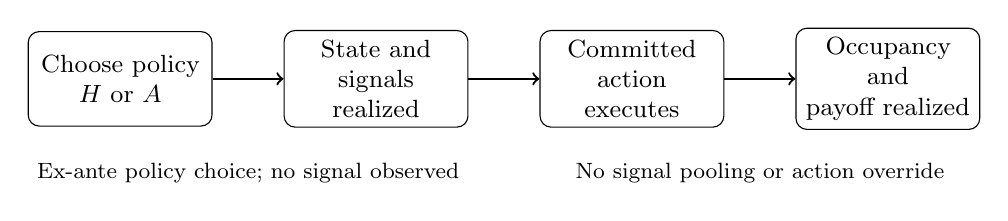
\begin{tikzpicture}[every node/.style={font=\small}]
\node[draw,rounded corners,align=center,text width=2.1cm,minimum height=1.2cm] (a) at (0,0) {Choose policy\\$H$ or $A$};
\node[draw,rounded corners,align=center,text width=2.1cm,minimum height=1.2cm] (b) at (3.25,0) {State and\\signals realized};
\node[draw,rounded corners,align=center,text width=2.1cm,minimum height=1.2cm] (c) at (6.5,0) {Committed\\action executes};
\node[draw,rounded corners,align=center,text width=2.1cm,minimum height=1.2cm] (d) at (9.75,0) {Occupancy and\\payoff realized};
\draw[->,thick] (a)--(b);\draw[->,thick] (b)--(c);\draw[->,thick] (c)--(d);
\node[align=center,font=\footnotesize] at (1.625,-1.2) {Ex-ante policy choice; no signal observed};
\node[align=center,font=\footnotesize] at (8.125,-1.2) {No signal pooling or action override};
\end{tikzpicture}
\caption{Timing of the policy-commitment game. The restriction on downstream execution defines the scope of the equilibrium theorem.}\label{fig:timing}
\end{figure}

\section{Symmetric adoption and efficiency}
Let $p\in[0,1]$ be the common independent probability of choosing $A$, and let $w(p)=\E[W]/N$. Define
\begin{align}
 q_{HH}&=a^2+(1-a)^2,&q_{HA}&=ab+(1-a)(1-b),&q_{AA}&=1,\label{eq:pairs}\\
 L&=c(N-1),&\delta&=d(b-a),\\
 \alpha&=q_{HA}-q_{HH}=(b-a)(2a-1),&
 \beta&=1-2q_{HA}+q_{HH}.\label{eq:constants}
\end{align}
Both $\alpha$ and $\beta$ are positive. For $\beta$, writing $t=2a-1$ and $s=2b-1$ gives $\beta=(1+t^2-2ts)/2>(1-t)^2/2>0$.
Pairwise conditioning and Proposition~\ref{prop:decomp} give
\begin{align}
 q(p)&=(1-p)^2q_{HH}+2p(1-p)q_{HA}+p^2
      =q_{HH}+2\alpha p+\beta p^2,\label{eq:q}\\
 w(p)&=v_0+da+\delta p-Lq(p).\label{eq:w}
\end{align}
Against opponents using adoption probability $p$, the expected gain from selecting $A$ rather than $H$ is
\begin{equation}\label{eq:gain}
 D(p)=\delta-L\bigl[\alpha+\beta p\bigr].
\end{equation}
Indeed, each opponent using $H$ adds collision difference $\alpha$, and each using $A$ adds $1-q_{HA}=\alpha+\beta$.

\begin{theorem}[Symmetric equilibrium and expected loss]\label{thm:mixed}
Under Assumption~\ref{ass:timing}, the unique symmetric adoption probability in Nash equilibrium is
\begin{equation}\label{eq:pE}
 p_E=\clip\left(\frac{\delta/L-\alpha}{\beta},0,1\right),
\end{equation}
where $\clip(x,0,1)=\min\{1,\max\{0,x\}\}$. If
\begin{equation}\label{eq:interior}
 L\alpha<\delta<L(\alpha+\beta),
\end{equation}
the equilibrium is interior, and every participant has the same expected payoff satisfying
\begin{equation}\label{eq:loss}
 w(p_E)-w(0)=-L\alpha p_E<0.
\end{equation}
\end{theorem}
\begin{proof}
Equation~\eqref{eq:gain} is strictly decreasing in $p$. An interior symmetric mixture requires indifference, $D(p)=0$, which yields \eqref{eq:pE}. If $D(0)\leq0$, $p=0$ is the symmetric equilibrium; if $D(1)\geq0$, $p=1$ is. These statements include the endpoint indifference cases and establish uniqueness among symmetric profiles. At an interior equilibrium, $\delta=L(\alpha+\beta p_E)$. Subtracting $w(0)$ from \eqref{eq:w} and substituting this equality yields
\[
 \delta p_E-L(2\alpha p_E+\beta p_E^2)=-L\alpha p_E.
\]
Symmetry gives equal ex-ante payoffs. Strict negativity follows from $L,\alpha,p_E>0$.
\end{proof}
The equilibrium is not claimed to be unique among asymmetric profiles. The theorem concerns ex-ante expectations, not a Pareto comparison in every realization. Moreover, a large loss under forced full adoption should not be substituted for the equilibrium loss when full adoption is not individually stable.

\begin{proposition}[Restricted efficient adoption]\label{prop:social}
The adoption probability maximizing average payoff among symmetric independent lotteries is
\begin{equation}\label{eq:pS}
 p_S=\clip\left(\frac{\delta/L-2\alpha}{2\beta},0,1\right).
\end{equation}
If both $p_E$ and $p_S$ are interior, $p_E-p_S=\delta/(2L\beta)>0$.
\end{proposition}
\begin{proof}
From \eqref{eq:w}, $w'(p)=\delta-2L(\alpha+\beta p)$ and $w''(p)=-2L\beta<0$. The unique constrained maximizer is \eqref{eq:pS}. Subtracting the two interior expressions proves the final statement.
\end{proof}
The qualifier ``restricted'' matters. A planner could coordinate adopter identities or actions rather than use independent lotteries. The next section treats the first of these alternatives.

\section{Finite populations and pure adoption}
Suppose exactly $m$ named participants adopt $A$. Let $\bar w_m$ denote expected average payoff under this deterministic policy profile. Ordered-pair counting yields
\begin{equation}\label{eq:fixed}
 \bar w_m=v_0+da+\frac{\delta m}{N}
 -\frac{c}{N}\left[(N-m)(N-m-1)q_{HH}
 +2m(N-m)q_{HA}+m(m-1)\right].
\end{equation}
Expanding \eqref{eq:fixed} gives the useful expression
\begin{equation}\label{eq:fixedchange}
 \bar w_m-w(0)=\frac{m}{N}
 \left[\delta-c\{2(N-1)\alpha+(m-1)\beta\}\right].
\end{equation}
Against exactly $k$ adopting opponents, the private gain from adoption is
\begin{equation}\label{eq:Dk}
 D_k=\delta-c\bigl[(N-1)\alpha+k\beta\bigr].
\end{equation}

\begin{proposition}[Pure equilibrium counts]\label{prop:pure}
An interior adopter count $m\in\{1,\ldots,N-1\}$ supports a pure Nash equilibrium if and only if
\begin{equation}\label{eq:pure}
 m-1\leq T\leq m,\qquad
 T=\frac{\delta/c-(N-1)\alpha}{\beta}.
\end{equation}
The boundary count $m=0$ is an equilibrium if $D_0\leq0$, and $m=N$ is an equilibrium if $D_{N-1}\geq0$. If $(N-1)\alpha>\beta$, every interior pure equilibrium has $\bar w_m<w(0)$.
\end{proposition}
\begin{proof}
A non-adopter faces $m$ adopting opponents and does not want to adopt if $D_m\leq0$. An adopter faces $m-1$ adopting opponents and does not want to leave if $D_{m-1}\geq0$. Substitution of \eqref{eq:Dk} gives \eqref{eq:pure}. The same logic proves the boundary conditions. At an interior pure equilibrium, $\delta\leq c[(N-1)\alpha+m\beta]$. Substituting this bound into \eqref{eq:fixedchange} gives
\[
 \bar w_m-w(0)\leq\frac{cm}{N}\bigl[\beta-(N-1)\alpha\bigr]<0.
\]
\end{proof}
For noninteger $T$ in the interior range, the equilibrium count is $\lceil T\rceil$; an integer threshold can support two adjacent counts. The identities of adopters need not be unique. Proposition~\ref{prop:pure} supplies a sufficient condition under which the expected loss is not an artifact of symmetric mixed strategies.

\begin{proposition}[Coordinating adopter counts]\label{prop:count}
For an integer $m$ and $p=m/N$,
\begin{equation}\label{eq:coord}
 \bar w_m-w(p)=c\beta p(1-p)\geq0.
\end{equation}
A count maximizing \eqref{eq:fixed} is obtained by checking the feasible integers adjacent to the clipped continuous maximizer
\begin{equation}
 m_S^{\mathrm{cont}}=\clip\left(
 \frac12+\frac{\delta/c-2(N-1)\alpha}{2\beta},0,N\right).
\end{equation}
\end{proposition}
\begin{proof}
Substitute $p=m/N$ into \eqref{eq:w} and subtract from \eqref{eq:fixedchange}. The difference is $c\beta(m/N-m^2/N^2)$. Alternatively, independent adoption gives a binomial count $M$ with variance $Np(1-p)$; the quadratic term in \eqref{eq:fixedchange} implies a Jensen gap $c\beta\operatorname{Var}(M)/N$. Differentiating the concave quadratic in $m$ gives the stated continuous maximizer, after which adjacent integers suffice.
\end{proof}
Count coordination is not necessarily incentive compatible. It is an allocation benchmark, not a decentralized equilibrium or an implementable mechanism without additional incentives.

\section{Partial commonality and the role of adaptation}
\subsection{A controlled dependence comparison}
Let $r\in[0,1]$. With probability $r$, all adopters share a single Bernoulli correctness draw with parameter $b$; otherwise each adopter receives an independent Bernoulli draw with the same parameter. The regime draw is independent of signals and adoption. Private signals remain conditionally independent. Marginal accuracy stays at $b$, while
\begin{align}
 q_{AA}(r)&=b^2+(1-b)^2+2rb(1-b),\\
 \beta(r)&=q_{AA}(r)-2q_{HA}+q_{HH}
           =2(b-a)^2+2rb(1-b)>0.\label{eq:betar}
\end{align}
All symmetric-adoption formulas continue to hold with $\beta(r)$, because they use only the pairwise collision probabilities. At fixed $p>0$,
\begin{equation}
 \frac{\partial w(p,r)}{\partial r}=-2Lp^2b(1-b)<0.
\end{equation}
At an interior equilibrium, however,
\begin{equation}
 \frac{\mathrm d p_E(r)}{\mathrm d r}
 =-\frac{(\delta/L-\alpha)\,2b(1-b)}{\beta(r)^2}<0.
\end{equation}
Together with \eqref{eq:loss}, this implies that equilibrium payoff increases with $r$ on an interior branch: stronger dependence discourages enough adoption to reduce the equilibrium loss. This local comparative static should not be extrapolated across boundary regimes without using the clipped equilibrium expression. Fixed-adoption and endogenous-adoption comparisons answer different questions.


\begin{figure}[tb]
\centering
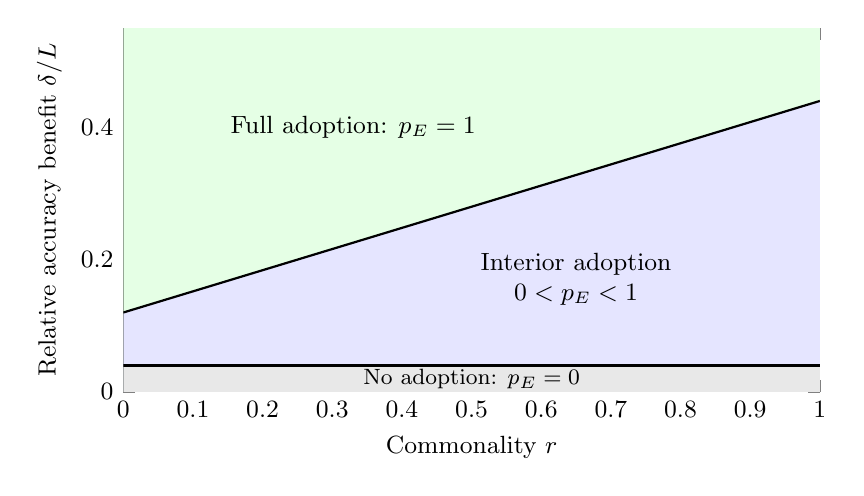
\begin{tikzpicture}
\begin{axis}[width=.86\linewidth,height=6.2cm,xmin=0,xmax=1,ymin=0,ymax=.55,xlabel={Commonality $r$},ylabel={Relative accuracy benefit $\delta/L$},tick label style={font=\small},label style={font=\small}]
\addplot[draw=none,fill=gray!18] coordinates {(0,0)(1,0)(1,.04)(0,.04)}\closedcycle;
\addplot[draw=none,fill=blue!10] coordinates {(0,.04)(1,.04)(1,.44)(0,.12)}\closedcycle;
\addplot[draw=none,fill=green!10] coordinates {(0,.12)(1,.44)(1,.55)(0,.55)}\closedcycle;
\addplot[black,thick] coordinates {(0,.04)(1,.04)};
\addplot[black,thick] coordinates {(0,.12)(1,.44)};
\node[font=\footnotesize] at (axis cs:.5,.019){No adoption: $p_E=0$};
\node[font=\small,align=center] at (axis cs:.65,.17){Interior adoption\\$0<p_E<1$};
\node[font=\small] at (axis cs:.33,.40){Full adoption: $p_E=1$};
\end{axis}
\end{tikzpicture}
\caption{Equilibrium adoption regions with $a=0.6$ and $b=0.8$. The lower boundary is $\delta/L=\alpha=0.04$ and the upper boundary is $\delta/L=\alpha+\beta(r)=0.12+0.32r$. Boundary indifference is included in the clipped rule. The interior region satisfies the strict loss result.}\label{fig:regions}
\end{figure}

\begin{figure}[tb]
\centering
\begin{tikzpicture}
\begin{axis}[width=.86\linewidth,height=6.2cm,xmin=0,xmax=1,ymin=-.09,ymax=.10,ytick={-.08,-.04,0,.04,.08},scaled y ticks=false,yticklabel style={/pgf/number format/fixed,/pgf/number format/precision=2},xlabel={Commonality $r$},ylabel={Payoff change relative to private only},grid=major,grid style={gray!20},legend style={font=\footnotesize,at={(.98,.98)},anchor=north east},tick label style={font=\small},label style={font=\small}]
\addplot[blue!65!black,thick] table[x=r,y=fixed]{commonality.dat};
\addlegendentry{Fixed adoption $p=0.40505$}
\addplot[black,dashed,thick] table[x=r,y=endogenous]{commonality.dat};
\addlegendentry{Endogenous adoption $p_E(r)$}
\addplot[gray,dotted] coordinates {(0,0)(1,0)};
\end{axis}
\end{tikzpicture}
\caption{Comparative statics at fixed and endogenous adoption, holding marginal accuracies and the numerical calibration fixed. Greater commonality always lowers payoff at fixed adoption. On the interior-equilibrium branch it raises payoff by discouraging adoption. The transition is at $r^*=203/792\approx0.2563$, where $\delta/L=\alpha+\beta(r^*)$; full adoption ceases to be an equilibrium above this threshold.}\label{fig:commonality}
\end{figure}

\subsection{Bayesian implementation after observing both signals}
The policy-commitment restriction can be relaxed for the interior symmetric outcome under a precise information structure. Suppose every participant observes its own pair $(H_i,A_i)$ before choosing an action, but not the state, the commonality regime, others' signals, or realized occupancy. Signal access is free; the joint signal law is as above, with label symmetry and conditional independence of private signals. Participants may choose any randomized mapping from their own pair to the two actions. Independent randomization is available. This is a simultaneous Bayesian action game, rather than a sequential game with observable histories.

\begin{proposition}[Post-signal implementation]\label{prop:obedience}
Fix $r\in[0,1]$ and suppose $0<p_E(r)<1$. The following strategy is a symmetric Bayesian Nash equilibrium: follow the recommendation when $H_i=A_i$; when they disagree, follow $A_i$ with probability $p_E(r)$ and $H_i$ otherwise. Its joint action distribution and expected payoff coincide with the symmetric mixed policy outcome. Thus \eqref{eq:loss} also holds in this specified Bayesian game.
\end{proposition}
\begin{proof}
Against opponents using the proposed strategy with probability $p$, let $G_A$ and $G_H$ be unconditional expected gains from following the respective signal instead of choosing its opposite. Pairwise conditioning gives
\begin{align}
 G_A&=d(2b-1)-L\{(1-p)(2q_{HA}-1)+p(2q_{AA}(r)-1)\},\\
 G_H&=d(2a-1)-L\{(1-p)(2q_{HH}-1)+p(2q_{HA}-1)\}.
\end{align}
Their difference is $G_A-G_H=2D(p,r)$, where $D(p,r)=\delta-L\{\alpha+\beta(r)p\}$. Write $\Delta_{=}$ for the conditional gain from following the common recommendation on agreement, and $\Delta_{\ne}$ for the gain from choosing $A_i$ rather than $H_i$ on disagreement. Label symmetry makes each gain identical for the two labeled signal pairs in its event. The agreement event has probability $q_{HA}$, and adding or subtracting the two unconditional gains yields
\begin{equation}\label{eq:conditionalgains}
 \Delta_{=}=\frac{G_A+G_H}{2q_{HA}},\qquad
 \Delta_{\ne}=\frac{D(p,r)}{1-q_{HA}}.
\end{equation}
At an interior equilibrium $D(p_E,r)=0$. Substituting
$d=L\{\alpha+\beta(r)p_E\}/(b-a)$ and using \eqref{eq:betar} gives
\begin{equation}\label{eq:obedience}
 G_A=G_H=\frac{2Lrb(1-b)(2a-1)}{b-a}\,p_E\geq0.
\end{equation}
Thus agreement is followed optimally (strictly when $r>0$), and either action is optimal on disagreement. These exhaust the four possible private signal types and all binary-action deviations. Drawing an independent policy coin before signals, or drawing the same coin only on disagreement, produces the same actions conditional on every signal realization. The induced joint distribution and payoff therefore coincide.
\end{proof}
This is an existence result, not a uniqueness or learning-stability result. It does not cover richer observations, public disclosure of the commonality regime, communication, costly information acquisition, or unrestricted recommendation design. It also does not establish post-signal implementation of the asymmetric pure policy equilibria. Under the same interior condition, the private-only baseline is itself an equilibrium when only $H_i$ is available: following it yields conditional gain $(2a-1)[d-L(2a-1)]>0$. The comparison can therefore be read as equilibrium deterioration following expanded signal access within these specific games.

\subsection{Execution outside the policy menu}
If participants observe true opportunity values and can revise actions, they play a different congestion game. Let $k$ choose the good opportunity. When both opportunities are occupied, the no-switch conditions are
\begin{equation}\label{eq:action}
 c(2k-N-1)\leq d\leq c(2k-N+1).
\end{equation}
The left inequality compares a good-opportunity user's current payoff with its payoff after switching; the right compares an other-opportunity user's payoff with entry into the good opportunity. If $d\geq c(N-1)$, all participants selecting the good opportunity is an action equilibrium. A coordinated full-information planner instead maximizes
\begin{equation}
 Nv_0+dk-c\{k(k-1)+(N-k)(N-k-1)\},
\end{equation}
whose continuous optimum is $k=N/2+d/(4c)$, clipped to $[0,N]$ and then checked at adjacent integers. Full information and efficient coordination are distinct. These full-information benchmarks differ from both the policy game and Proposition~\ref{prop:obedience}; they demonstrate why the allowed policy set must be stated.

\section{Computational verification}
\subsection{Design}
The numerical example uses
\[
 N=100,\quad a=0.60,\quad b=0.80,\quad v_0=9,
 \quad d=2,\quad c=0.02.
\]
Thus $L=1.98$, $\alpha=0.04$, and $\beta=0.40$. The parameters illustrate an interior adoption equilibrium and a positive restricted efficient adoption rate; they are not estimated from a market. Python and NumPy generate 50,000 independent markets for each of four adoption probabilities, using generator seed 20261105 and batches of 1,000. Each market draws $N$ independent adoption indicators, $N$ private correctness indicators, and one common correctness indicator. The good opportunity can be assigned a fixed label without loss because the two state labels have symmetric payoffs.

Within each market, the realized mean payoff is computed from occupancy. Monte Carlo standard errors use the sample variance of market means divided by the number of markets. Individual outcomes within a market are dependent and are not treated as independent samples. The four conditions use successive unpaired draws of the same generator.

The implementation also performs exact enumeration for $N=4$ at $p\in\{0,0.17,0.5,1\}$, checks 6,564 interior cases on a parameter grid, and verifies 1,404 finite-count configurations with Python's exact rational arithmetic. The latter checks use three population sizes, three signal pairs, four cost values, and every feasible adopter count. A separate exact state-and-signal enumeration checks Proposition~\ref{prop:obedience} in 37 interior parameter cases (148 labeled own-signal types), plus 16 off-equilibrium types. These are numerical and algebraic consistency checks, not a proof-assistant certification or empirical validation.

\subsection{Results}
\begin{table}[tb]
\centering
\small
\caption{Expected payoff and Monte Carlo verification. Payoffs are arbitrary model units per participant; each simulated condition uses 50,000 independent markets.}\label{tab:main}
\begin{tabular}{lrrrr}
\toprule
Regime & $p$ & Exact & Monte Carlo & Standard error\\
\midrule
Private only & 0.0000 & 9.17040 & 9.17024 & 0.000271 \\
Optimal independent adoption & 0.1525 & 9.18883 & 9.18908 & 0.000434 \\
Mixed adoption equilibrium & 0.4051 & 9.13832 & 9.14127 & 0.001139 \\
Full common adoption & 1.0000 & 8.62000 & 8.62372 & 0.003565 \\
\bottomrule
\end{tabular}

\end{table}

The symmetric equilibrium adoption probability is $p_E=0.4050505$, whereas $p_S=0.1525253$. The exact loss at equilibrium is $0.03208$ per participant relative to the private-only baseline, approximately $0.35\%$ of baseline payoff. Restricted efficient adoption gains $0.0184251$ per participant. These percentages have no direct monetary or macroeconomic interpretation. Full adoption has a larger loss but is not an adoption equilibrium for this calibration.

\begin{figure}[tb]
\centering
\begin{tikzpicture}
\begin{axis}[width=.88\linewidth,height=6cm,xlabel={Common-policy adoption probability $p$},ylabel={Payoff change relative to $p=0$},xmin=0,xmax=1,ymin=-.58,ymax=.06,grid=major,grid style={gray!20},tick label style={font=\small},label style={font=\small}]
\addplot[blue!65!black,thick] table[x=p,y=change]{curve.dat};
\addplot[only marks,mark=*,black] coordinates {(.15252525,.01842505) (.40505051,-.03208)};
\node[anchor=south west,font=\small] at (axis cs:.15252525,.01842505){$p_S$};
\node[anchor=north east,font=\small] at (axis cs:.40505051,-.03208){$p_E$};
\end{axis}
\end{tikzpicture}
\caption{Exact payoff change from \eqref{eq:w}. The voluntary equilibrium lies beyond the adoption level maximizing expected payoff among independent symmetric lotteries.}\label{fig:curve}
\end{figure}

The finite game has pure equilibria with 41 adopters, yielding mean payoff $9.138256$, also below the private-only baseline $9.1704$. The best fixed count is 16, yielding $9.189856$. Thus the qualitative loss is not created solely by the randomness of the symmetric mixture. The small advantage of fixed-count coordination over independent adoption is consistent with Proposition~\ref{prop:count}.

Exact enumeration differs from the analytical formula by at most $2.85\times10^{-14}$ in floating-point computation. All four Monte Carlo discrepancies are below three standard errors. The mixed-equilibrium simulated mean is 2.59 standard errors above its expectation; the seed was retained rather than selected for closer agreement. Table~\ref{tab:main} reports Monte Carlo uncertainty, not uncertainty about empirical parameters.

For a countercase, keep common-policy marginal accuracy at $b=0.8$ but set $r=0$. At full adoption, $q_{AA}=0.68$, so expected payoff is $9.2536$, exceeding the private-only baseline. In the fully informed action game, all participants choosing the good opportunity is an equilibrium with payoff $9.02$ because $d=2>c(N-1)=1.98$. A coordinated full-information allocation with 75 participants in the good opportunity yields $9.27$. These comparisons involve different information and coordination constraints and should not be presented as estimates of one intervention.


\subsection{Worked exact example}
For the calibration, $a=3/5$, $b=4/5$, $c=1/50$, and $d=2$. Direct substitution gives
\[
 q_{HH}=\frac{13}{25},\quad q_{HA}=\frac{14}{25},\quad
 \alpha=\frac1{25},\quad\beta=\frac25,\quad
 L=\frac{99}{50},\quad\delta=\frac25.
\]
The symmetric equilibrium and restricted optimum are therefore
\[
 p_E=\frac{401}{990},\qquad p_S=\frac{151}{990},\qquad
 w(p_E)-w(0)=-\frac{401}{12500}=-0.03208.
\]
For pure adoption, $T=401/10=40.1$. The only interior equilibrium count is consequently $m=41$, since $40\leq40.1\leq41$. The sufficient loss condition holds because $(N-1)\alpha=99/25>2/5=\beta$. The fixed-count continuous optimum is $15.6$; evaluating the adjacent integers selects $m=16$. For post-signal implementation at $r=1$, $G_A=G_H=802/3125$, so the gain on agreement is $\Delta_{=}=401/875>0$ and on disagreement $\Delta_{\ne}=0$. Exact conditional enumeration verifies both statements. This example illustrates the proofs with exact fractions rather than relying on a simulation to establish the sign.

\section{Discussion and limitations}
The analysis identifies a conditional externality from adopting common executable advice. Better marginal signal accuracy does not determine the value of a population-wide deployment: dependence and congestion also matter. Nevertheless, commonality need not be harmful. With zero congestion, more accurate policies improve payoffs. At $a=1/2$, the interior-equilibrium loss vanishes because $\alpha=0$. If capacity scales with population so that $c=\kappa/(N-1)$, the factor $L$ remains fixed and there is no mechanical population-size amplification.

The baseline model restricts policy execution. Proposition~\ref{prop:obedience} establishes that the interior symmetric outcome can also be sustained when agents optimize after observing both of their signals. Its private information structure is essential; richer observations and recommendation design remain outside the result. Homogeneous preferences and linear, symmetric congestion are further restrictions. Heterogeneous tasks and nonlinear costs alter the collision-to-payoff mapping. Private errors are independent conditional on the state; real human and algorithmic judgments can share errors even without a common provider.

The computational results are internal verification only. There are no live language-model calls, human participants, external datasets, or estimates of economy-wide losses. Nor does this static model demonstrate dynamic instability or chaos. A credible application would measure resource costs and manipulate evidence overlap, policy overlap, and congestion feedback separately. Group-level randomization is needed because decisions interact within markets; treating agents as independent observational units would understate uncertainty.

Publication-level novelty remains a separate question from mathematical validity. The broad mechanism is already established, and full-text comparison with the recent firm-entry work remains outstanding. The present contribution is a compact, explicit model with finite-population comparisons and a reproducible verification record. Its value as a journal contribution requires assessment against the closest literature, not merely successful compilation or numerical agreement.

\section{Conclusion}
A more accurate common policy can attract voluntary adoption while reducing expected participant payoff. In the restricted binary-signal game, the loss has a simple expression and survives at pure finite-population equilibria under a sufficient condition. Coordinating adopter counts improves outcomes relative to independent adoption with the same expected count. Partial-commonality analysis further shows that fixed-adoption and endogenous-adoption comparisons can point in opposite directions. These results support evaluating shared advice at the population level while retaining explicit assumptions about capacity, dependence, and the ability to revise actions.

\section*{Research transparency}
\paragraph{Code and data.} The manuscript source, analysis code, and synthetic results are available at \url{https://github.com/triggeredcode/shared-intelligence-competing-decisions}. No real-world observations or live-model experiments are reported.
\paragraph{AI assistance.} AI was used in model development, analysis, coding, and manuscript preparation.
\paragraph{Status.} This is a working paper and has not been peer reviewed.

\bibliographystyle{plainnat}
\bibliography{references}
\end{document}
